\documentclass[12pt,a4paper]{article}
\usepackage[a4paper, margin=2.5cm]{geometry}
\usepackage[utf8]{inputenc}
\usepackage[T1]{fontenc}
\usepackage{lmodern}
\usepackage{amsmath, amssymb, amsthm, mathtools}
\usepackage{booktabs, array}
\usepackage{graphicx, xcolor}
\usepackage{caption, subcaption}
\usepackage{hyperref}
\hypersetup{
  colorlinks=true,
  linkcolor=blue!70!black,
  citecolor=blue!70!black,
  urlcolor=blue!70!black
}
\usepackage{natbib}
\usepackage{setspace}
\onehalfspacing

\newcommand{\bint}{\beta_{\text{int}}}
\newcommand{\E}{\mathbb{E}}
\newcommand{\R}{\mathbb{R}}
\newcommand{\N}{\mathbb{N}}

\theoremstyle{plain}
\newtheorem{proposition}{Proposition}
\newtheorem{theorem}{Theorem}
\newtheorem{lemma}{Lemma}
\theoremstyle{definition}
\newtheorem{definition}{Definition}
\newtheorem{example}{Example}
\newtheorem{assumption}{Assumption}

\title{A time-varying-parameter state-space approach to sparse-event survival modelling: methodological design, out-of-sample performance, and application to hydrogen project implementation-risk}

\author{Sake Saakstra\thanks{Vrije Universiteit Amsterdam. Email: \texttt{s.saakstra@vu.nl}. I am grateful to Siem Jan Koopman, Nadine Ketel, and seminar participants at VU Amsterdam for valuable feedback. All errors are mine.}
\and Siem Jan Koopman\thanks{Vrije Universiteit Amsterdam and Tinbergen Institute. \emph{TBC --- subject to co-author confirmation.}}}

\date{First draft: \today}

\begin{document}

\maketitle

\begin{abstract}
\noindent
We propose a time-varying-parameter (TVP) state-space approach to survival modelling under sparse-event data conditions, in which the conditional hazard depends on a generative-process parameter whose evolution is driven by the score of the predictive likelihood. The Score-Driven Generalized Autoregressive Score (GAS) specification of \cite{creal2013generalized} provides a parsimonious and asymptotically optimal mechanism for parameter time-variation, requiring only the score and a one-parameter persistence specification.

Three rival TVP specifications are compared: M1 with constant parameter, M2 with parameter-driven block-step transitions, and M3 with observation-driven GAS persistence. The three are tested for out-of-sample forecast accuracy via three independent designs --- a 75-25 time split, 5-fold within-project block cross-validation, and rolling one-step-ahead full-sample prediction. Significance is assessed by the Diebold-Mariano-Harvey-Leybourne-Newbold test on per-observation Bernoulli log-loss. The Score-Driven specification wins uniformly in point estimates across all three designs and is the unique element of the Hansen-Lunde-Nason Model Confidence Set at $\alpha = 0.10$ under the rolling-one-step design. The DM-HLN test statistics for M3 versus M1 and M3 versus M2 are $+5.59$ and $+4.80$ respectively ($p < 0.0001$) under the rolling-window design, with the largest performance gain concentrated in the 2023 cancellation wave where the carbon-conditional mechanism intensifies.

The methodology is applied to a sample of 714 hydrogen projects with 43 failure events, drawn from the v7 working-paper sample of \cite{saakstra2025v7}, spanning announcement-stage status from 2010--2026. The aggregated person-year panel contains 4,162 observations, reduced to 34 Binomial cells by year-and-technology aggregation. The interaction coefficient $\bint(t)$ governing the carbon-conditional Blue/Green hazard differential is estimated to intensify from $-0.46$ in 2010 to $-1.49$ in 2024 under the score-driven specification, with a structural break detected around 2020. The Score-Driven TVP approach is a useful general-purpose methodology for survival modelling in domains with sparse-event data, sample-window dependence concerns, and reasonable suspicion of structural-break dynamics.

\medskip
\noindent\textbf{JEL classification}: C32, C41, Q42

\noindent\textbf{Keywords}: time-varying parameter; score-driven model; state-space; survival modelling; Diebold-Mariano test; hydrogen
\end{abstract}

\section{Introduction}
\label{sec:intro}

Survival modelling under sparse-event conditions presents two related identification challenges. First, when the rate of events per period is low, the unconditional hazard is poorly estimated and inference about technology- or sector-specific differentials becomes sample-size-bound. Second, when the conditioning relationship itself may be evolving --- because the underlying economic environment is non-stationary, because a policy regime is shifting, or because the relevant institutional structure is recalibrating --- the standard time-invariant proportional-hazards specification can mask a substantial fraction of the true information content of the data. The conventional remedy for the first problem is to expand the sample window, but doing so often compounds the second problem: a wider window is more likely to span periods of structural change. The two problems pull in opposite directions, and any econometric strategy that resolves them must navigate the trade-off explicitly.

This paper develops one such strategy. We propose a time-varying-parameter (TVP) state-space formulation in which the conditioning coefficient governing the technology-specific hazard differential is permitted to evolve over time according to a score-driven recursion. The Score-Driven Generalized Autoregressive Score (GAS) framework of \cite{creal2013generalized} provides three properties that are well-suited to the sparse-event survival problem. First, the recursion is driven by the score of the predictive log-likelihood, which under a one-step optimal scoring rule maximises the per-observation predictive Kullback-Leibler divergence and is asymptotically efficient \citep{harvey2013dynamic, blasques2015robust}. Second, the parsimony of the GAS specification --- a single persistence parameter on top of any time-invariant structure --- avoids the over-parametrisation that random-walk-driven TVP specifications incur in finite samples. Third, the score-driven structure can be integrated naturally with the Bayesian state-space inference machinery of \cite{durbin2012time}, supporting joint posterior inference on both the time-varying parameter trajectory and the static hyperparameters.

The methodological contribution of this paper has three parts. First, we develop the score-driven TVP specification in the context of a Bernoulli-likelihood hazard model, deriving the GAS recursion explicitly and providing prior structure for the static parameters. We show that the resulting specification is well-identified under standard regularity conditions and that the prior structure can be calibrated to deliver shrinkage toward a constant-parameter null without violating the asymptotic efficiency of the score-driven recursion. Second, we provide a rigorous out-of-sample comparison framework that contrasts the GAS specification against the two principal alternatives in the TVP literature --- constant-parameter (M1) and parameter-driven block transitions (M2). The comparison is conducted across three independent test designs: a 75-25 time split, 5-fold within-project block cross-validation, and a rolling one-step-ahead full-sample comparison. Statistical significance is assessed using the \cite{diebold1995comparing} test with the small-sample correction of \cite{harvey1997testing}, and joint statistical containment is established via the simplified \cite{hansen2011model} Model Confidence Set procedure. The use of multiple independent test designs is essential under sparse-event conditions, where any single design can be vulnerable to the temporal location of the events relative to the train-test boundary.

Third, the methodology is applied to a substantive application of independent interest: the carbon-conditional implementation risk of hydrogen projects. The application uses a sample of 714 hydrogen projects with 43 failure events drawn from the v7 working-paper precursor sample, spanning announcement-stage status from 2010 through early 2026. The aggregated person-year panel contains 4{,}162 observations, reduced to 34 Binomial cells by year-and-technology aggregation. The binary outcome is a failure indicator aggregating cancellation, decommissioning, and on-hold transitions, and the principal time-varying parameter is the interaction coefficient $\bint(t)$ governing the Blue-versus-Green hazard differential conditional on the EUA carbon price. Under the score-driven specification, $\bint(t)$ is estimated to intensify monotonically from $-0.46$ in 2010 to $-1.49$ in 2024, with a discernible structural break around 2020 corresponding to the European Green Deal acceleration of EUA prices. The constant-parameter specification yields a sample-average estimate of $\hat{\bint} = -1.37$ that masks this intensification.

The substantive result --- that the Blue-versus-Green hazard differential has intensified over the EUA-price-rise period --- is consistent with a real-options interpretation in which the differential carbon payoff of clean over fossil hydrogen has grown as the EUA price has risen, raising the optimality threshold for cancellation among blue projects relative to green projects. This interpretation is consistent with the comparative-statics implications of the standard \cite{dixit1994investment} irreversibility framework when applied to the carbon-conditional payoff structure, and provides a natural test of the carbon-price-mediated mechanism in the contemporary clean-hydrogen environment.

The methodological contribution of the paper is, however, the principal product. The GAS-TVP specification we develop and the OOS-comparison framework we apply are general-purpose tools for survival modelling under conditions of sparse events and potential parameter instability. Domains in which the methodology should be useful include early-stage venture failure analysis, project-finance termination, clinical-trial dropout, and any other survival application in which the conditional hazard may be evolving and the events themselves are sparse on the per-period margin. We provide full reproducibility code at \texttt{[github.com/SakeSaak/paper1\_tvp]}, including the MCMC implementation, the DM-test routines, and the rolling-window cross-validation framework.

The remainder of the paper is organised as follows. Section~\ref{sec:literature} reviews the related literature on time-varying-parameter econometrics, score-driven models, survival modelling under sparse events, and the Diebold-Mariano-Hansen-Lunde-Nason inferential framework. Section~\ref{sec:methodology} develops the methodological specification and the OOS-comparison procedure. Section~\ref{sec:data} describes the application data. Section~\ref{sec:results} reports the results, including the trajectory estimates, the OOS comparison, and the model-confidence-set inference. Section~\ref{sec:discussion} discusses the interpretation, the methodological lessons, and the limitations. Section~\ref{sec:conclusion} concludes.

\section{Related literature}
\label{sec:literature}

[To be drafted, $\sim 2$ pages. Source: thesis Chapter 2 Section ``Recent developments'' + score-driven literature.]

\section{Methodology}
\label{sec:methodology}

This section develops the time-varying-parameter state-space specification we propose, together with the out-of-sample inferential framework for comparing it against constant-parameter and parameter-driven alternatives. Section~\ref{sec:meth-setup} states the hazard model and the parametrisation of the time-varying coefficient. Section~\ref{sec:meth-specs} introduces three competing specifications of the time-variation structure. Section~\ref{sec:meth-bayes} describes Bayesian state-space inference under the three specifications. Section~\ref{sec:meth-oos} presents the out-of-sample comparison protocol, and Section~\ref{sec:meth-dm} develops the Diebold-Mariano test and the Model Confidence Set procedure.

\subsection{Hazard model and time-varying interaction parameter}
\label{sec:meth-setup}

Let $i \in \{1, \ldots, N\}$ index projects and $t \in \{1, \ldots, T\}$ index calendar years. Define the binary event indicator $y_{it} \in \{0, 1\}$, which equals one if project $i$ enters a failure state (cancellation, on-hold, or decommissioning) in year $t$ and zero otherwise. Projects that have already failed in an earlier year are removed from the at-risk set in subsequent years, and projects that have reached operational status are similarly removed. Let $\mathcal{A}_t \subseteq \{1, \ldots, N\}$ denote the at-risk set in year $t$.

The conditional probability of failure in year $t$ given the at-risk set and a vector of covariates $x_{it}$ is parametrised by a complementary log-log link of a linear index in the covariates:
\begin{equation}
\Pr(y_{it} = 1 \mid x_{it}, \mathcal{A}_t) = 1 - \exp\!\left[-\exp(\eta_{it})\right], \qquad i \in \mathcal{A}_t,
\label{eq:hazard}
\end{equation}
where $\eta_{it}$ is the linear predictor. The covariate vector $x_{it}$ contains a constant, a technology indicator $\text{Blue}_i$ (one if the project is Fossil-with-CCS and zero if Electrolysis), the contemporaneous EUA price $z_t$ (standardised), control covariates $C_{it}$ (log capacity, region fixed effects, year polynomial), and the interaction term $\text{Blue}_i \cdot z_t$:
\begin{equation}
\eta_{it} = \alpha + \beta_B \, \text{Blue}_i + \beta_Z \, z_t + \bint(t) \, \text{Blue}_i \cdot z_t + \gamma' C_{it}.
\label{eq:linear-predictor}
\end{equation}
The principal parameter of interest is the time-varying interaction coefficient $\bint(t)$, which governs the Blue-versus-Green hazard differential conditional on the EUA price. A negative value of $\bint(t)$ implies that the cancellation hazard of blue projects \emph{rises} with the EUA price relative to that of green projects, consistent with the carbon-conditional mechanism predicted by the real-options framework of \cite{dixit1994investment}. The remaining static parameters $(\alpha, \beta_B, \beta_Z, \gamma)$ are treated as time-invariant. The choice of complementary log-log over logit follows from the discrete-time-survival interpretation of \eqref{eq:hazard} as the discretisation of an underlying continuous-time hazard rate.

\begin{assumption}[Exogeneity of covariates]
\label{assn:exog}
The covariates $(x_{it})$ are strictly exogenous: conditional on $x_{it}$ and the at-risk set $\mathcal{A}_t$, the event indicator $y_{it}$ is independent of the failure outcomes of other projects at time $t$ and of the future paths of the covariates.
\end{assumption}

\begin{assumption}[Bernoulli likelihood]
\label{assn:bernoulli}
Given the parameters and the linear predictor \eqref{eq:linear-predictor}, the event indicators $y_{it}$ are conditionally independent Bernoulli random variables with success probability defined by \eqref{eq:hazard}.
\end{assumption}

\subsection{Three competing specifications of $\bint(t)$}
\label{sec:meth-specs}

We consider three specifications of the time-variation structure of $\bint(t)$, differing in the degree and form of permitted parameter evolution.

\paragraph{M1: Static.}
The first specification imposes time-invariance:
\begin{equation}
\bint(t) = \bint, \qquad t = 1, \ldots, T.
\label{eq:m1}
\end{equation}
This is the standard discrete-time-survival specification and serves as the baseline.

\paragraph{M2: Parameter-driven block transitions.}
The second specification permits $\bint(t)$ to take constant values within a small number of pre-specified blocks. Let $\{\mathcal{B}_b\}_{b=0}^B$ denote a partition of $\{1, \ldots, T\}$ into $B+1$ contiguous blocks:
\begin{equation}
\bint(t) = b_b \qquad \text{for } t \in \mathcal{B}_b, \quad b = 0, \ldots, B.
\label{eq:m2}
\end{equation}
The block boundaries are chosen to correspond to substantive policy regimes (the 2017--2018 Market Stability Reserve activation, the 2020 European Green Deal, and the 2023 IRA passage), yielding $B+1 = 4$ blocks in the application. The block coefficients $\{b_b\}$ are estimated jointly with the static parameters under a Gaussian random-walk prior for the parameter-driven structure: $b_b \mid b_{b-1} \sim \mathcal{N}(b_{b-1}, \tau^2)$, with $\tau$ a hyperparameter governing the magnitude of block-to-block variation. The static specification \eqref{eq:m1} is nested in M2 as the limit $\tau \to 0$.

\paragraph{M3: Observation-driven Score-Driven (GAS).}
The third specification permits $\bint(t)$ to evolve at the observation frequency via a score-driven recursion following \cite{creal2013generalized}. Let $\ell_t(\bint, \theta_{-})$ denote the per-period log-likelihood at time $t$ as a function of $\bint$ and the remaining parameters $\theta_{-} = (\alpha, \beta_B, \beta_Z, \gamma)$. The score with respect to $\bint(t)$ is
\begin{equation}
s_t = \left.\frac{\partial \ell_t(\bint, \theta_{-})}{\partial \bint}\right|_{\bint = \bint(t)} = \sum_{i \in \mathcal{A}_t} \left[y_{it} - 1 + \exp(-e^{\eta_{it}})\right] \frac{\partial \eta_{it}}{\partial \bint}.
\label{eq:score}
\end{equation}
The GAS recursion for the time-varying coefficient is
\begin{equation}
\bint(t+1) = \omega + \phi \cdot \bint(t) + \alpha_{\mathrm{gas}} \cdot s_t \cdot I_{t \mid t-1}^{-d},
\label{eq:gas}
\end{equation}
where $\omega$ is an unconditional mean parameter, $\phi$ is a persistence parameter, $\alpha_{\mathrm{gas}}$ is a score-loading parameter, and $I_{t \mid t-1}$ is the Fisher information of $\bint$ at time $t$ given information at time $t-1$. The scaling exponent $d \in \{0, 1/2, 1\}$ determines the metric in which the score acts on the parameter: $d = 1/2$ produces a score-driven recursion whose innovations have the asymptotic distribution of a standardised normal random variable under correct specification \citep{harvey2013dynamic}.

The static specification \eqref{eq:m1} is nested in M3 as the limit $\alpha_{\mathrm{gas}} = 0$. Under the conditions of \cite{blasques2015robust}, the score-driven recursion is the unique observation-driven scheme that yields a one-step optimal updating rule under the Kullback-Leibler scoring rule, providing an asymptotic-efficiency rationale for choosing M3 over the random-walk-driven alternative M2 when the underlying parameter trajectory is smooth.

\subsection{Bayesian state-space inference}
\label{sec:meth-bayes}

All three specifications are estimated by Hamiltonian Monte Carlo with the No-U-Turn sampler in PyMC 5.10. To stabilise the inference under the sparse-event likelihood and to facilitate comparability across the three specifications, the person-year panel is aggregated to a year-by-technology Binomial cell structure: for each year $t$ and technology level $j \in \{\text{Blue}, \text{Green}\}$, we compute the cell-level count of events $Y_{tj}$ and exposures $N_{tj}$, and treat $Y_{tj} \mid N_{tj}, p_{tj} \sim \text{Binomial}(N_{tj}, p_{tj})$ with success probability $p_{tj}$ given by \eqref{eq:hazard} evaluated at the cell-centroid covariate values. This aggregation reduces the $N = 4{,}162$ person-year observations to $T \times J = 17 \times 2 = 34$ Binomial cells, which is the form in which all three specifications are estimated.

The prior structure is as follows. For the static parameters: $\alpha \sim \mathcal{N}(0, 5^2)$, $\beta_B, \beta_Z \sim \mathcal{N}(0, 3^2)$, $\gamma_j \sim \mathcal{N}(0, 2^2)$. For M1: $\bint \sim \mathcal{N}(0, 3^2)$. For M2: $b_0 \sim \mathcal{N}(0, 3^2)$ and $b_b \mid b_{b-1} \sim \mathcal{N}(b_{b-1}, \tau^2)$ for $b = 1, \ldots, B$, with $\tau \sim \mathcal{H}\!\mathit{Cauchy}(0, 1)$. For M3: $\omega \sim \mathcal{N}(-1, 1^2)$ (centred near the M1 posterior mean to support comparability), $\phi \sim \text{Beta}(2, 2)$ shifted to $[-1, 1]$, $\alpha_{\mathrm{gas}} \sim \mathcal{H}\!\mathit{Cauchy}(0, 0.5)$, and the latent state initialisation $\bint(0) \sim \mathcal{N}(\omega / (1 - \phi), 1^2)$ at the unconditional mean implied by the recursion.

The sampler is run with four chains $\times$ 1{,}500 post-warm-up draws and target acceptance probability 0.99. Convergence is assessed by the Gelman-Rubin statistic ($\hat{R} < 1.01$ required), the effective sample size ($N_{\mathrm{eff}} > 400$ per chain required), and visual inspection of trace plots. The MCMC implementation, including the score function \eqref{eq:score} and the GAS recursion \eqref{eq:gas}, is provided in the replication package.

\subsection{Out-of-sample comparison protocol}
\label{sec:meth-oos}

The three specifications are compared on out-of-sample predictive accuracy across three independent test designs. The use of multiple designs is essential because under sparse-event conditions, any single design can be vulnerable to the temporal location of the events relative to the train-test boundary; the rolling-window design in particular concentrates a substantial fraction of the test-set events in a small number of years.

\paragraph{V1 --- Time-split (75-25).}
The full sample is split at the 75th percentile of the calendar-year distribution. The training set contains all project-year observations with $t \leq 2021$; the test set contains observations with $t > 2021$. Each specification is fit on the training set, and its predictive distribution is evaluated on the test set. The split contains five events in the training partition and 38 events in the test partition, reflecting the cancellation wave of 2023--2024.

\paragraph{V2 --- 5-fold within-project block cross-validation.}
The 714 projects are randomly partitioned into five folds of approximately equal size, holding constant the technology distribution within fold. For each fold $k$, the model is fit on the four other folds and the predictive distribution is evaluated on fold $k$. The procedure produces per-observation log-loss values that are aggregated across folds for the DM-test.

\paragraph{V3 --- Rolling one-step-ahead (full-sample).}
For each year $T_0 \in \{2021, 2022, 2023, 2024\}$, the model is fit on all observations with $t < T_0$ and the predictive distribution is evaluated on observations with $t = T_0$. This procedure simulates the real-time use of the model for one-year-ahead forecasting, in which the model is retrained as each new year of data becomes available. V3 is methodologically the strongest of the three designs, in that it most directly tests the predictive value of the time-varying-parameter specification under genuine sequential information flow.

The per-observation Bernoulli log-loss is the principal predictive scoring rule:
\begin{equation}
L_m(it) = -y_{it} \log(p_{m,it}) - (1-y_{it}) \log(1 - p_{m,it}),
\label{eq:logloss}
\end{equation}
where $p_{m,it}$ is the posterior-mean predictive probability under specification $m \in \{M_1, M_2, M_3\}$. Mean log-loss within design is computed as the average over all test-partition observations.

\subsection{Diebold-Mariano test and Model Confidence Set}
\label{sec:meth-dm}

For each pair of specifications $(A, B)$ within each test design, the loss differential
\begin{equation}
d_t^{AB} = L_A(t) - L_B(t)
\end{equation}
is computed for each test-partition observation $t$. Under the null hypothesis of equal predictive accuracy ($H_0: \E[d_t^{AB}] = 0$), the Diebold-Mariano test statistic of \cite{diebold1995comparing} is
\begin{equation}
DM^{AB} = \frac{\bar{d}^{AB}}{\sqrt{\widehat{\text{Var}}(\bar{d}^{AB})}},
\label{eq:dm}
\end{equation}
where $\bar{d}^{AB}$ is the sample mean of the loss differentials and $\widehat{\text{Var}}(\bar{d}^{AB})$ is the Newey-West HAC estimator with lag $\lfloor T_{\mathrm{test}}^{1/3} \rfloor$. Under $H_0$ and standard regularity conditions, $DM^{AB} \to_d \mathcal{N}(0, 1)$. In the small-sample setting that applies under sparse-event conditions, we use the \cite{harvey1997testing} correction:
\begin{equation}
DM_{\mathrm{HLN}}^{AB} = DM^{AB} \cdot \sqrt{\frac{T_{\mathrm{test}} + 1 - 2h + h(h-1)/T_{\mathrm{test}}}{T_{\mathrm{test}}}},
\label{eq:dmhln}
\end{equation}
where $h = 1$ for one-step-ahead forecasting and $T_{\mathrm{test}}$ is the number of test-partition observations. The HLN-corrected statistic is referred to a Student-$t$ distribution with $T_{\mathrm{test}} - 1$ degrees of freedom.

For joint inference across the three specifications, we apply the simplified \cite{hansen2011model} Model Confidence Set procedure with $\alpha = 0.10$. The procedure iteratively eliminates specifications whose average loss is statistically distinguishable from the lowest-loss specification, terminating when no further elimination is supported at the $\alpha$ level. The resulting confidence set $\mathcal{M}^*$ contains all specifications that cannot be statistically rejected as candidates for the best-loss model. A confidence set containing a single element provides the strongest possible inferential conclusion for OOS comparison under multiple competing specifications.

\section{Data}
\label{sec:data}

[To be drafted, $\sim 1$ page. Source: thesis Chapter 4 Section ``S\&P Global Commodity Insights data'' and v7 sample description.]

\section{Results}
\label{sec:results}

This section reports the results of the three competing specifications, the OOS comparison across the three test designs, the DM-HLN test inference, and the MCS containment. Section~\ref{sec:results-coef} presents the coefficient estimates and trajectory of $\bint(t)$ under each specification. Section~\ref{sec:results-oos} reports the OOS log-loss comparison. Section~\ref{sec:results-dm} reports the DM-HLN tests. Section~\ref{sec:results-mcs} reports the MCS containment. Section~\ref{sec:results-concentration} traces the source of the M3 advantage to the 2023 cancellation wave.

\subsection{Coefficient estimates and trajectory of $\bint(t)$}
\label{sec:results-coef}

Table~\ref{tab:results-coef} reports the posterior summary of $\bint$ (or its analogous structural parameter) under each of the three specifications.

\begin{table}[!htbp]
\centering
\caption{Posterior summary of $\bint$ under three specifications}
\label{tab:results-coef}
\begin{tabular}{lrrr}
\toprule
Specification & Posterior mean & 95\% credible interval & $N_{\text{eff}}$ \\
\midrule
M1 Static & $-1.37$ & $[-2.20, -0.49]$ & $5{,}872$ \\
M2 Block, $b_0$ (2010--2019) & $-1.52$ & $[-2.50, -0.62]$ & $4{,}910$ \\
M2 Block, $b_1$ (2020--2022) & $-1.74$ & $[-2.80, -0.75]$ & $5{,}108$ \\
M2 Block, $b_2$ (2023--2024) & $-0.75$ & $[-1.90, +0.43]$ & $4{,}680$ \\
M2 Block, $b_3$ (2025--2026) & $-2.06$ & $[-3.80, -0.62]$ & $3{,}910$ \\
M3 GAS, $\omega$ & $-1.61$ & $[-2.50, -0.69]$ & $5{,}401$ \\
M3 GAS, $\phi$ & $\phantom{-}0.92$ & $[\phantom{-}0.78, \phantom{-}0.99]$ & $4{,}212$ \\
M3 GAS, $\alpha_{\mathrm{gas}}$ & $\phantom{-}0.27$ & $[\phantom{-}0.08, \phantom{-}0.58]$ & $3{,}847$ \\
\bottomrule
\end{tabular}
\end{table}

The M1 static posterior mean of $-1.37$ is the sample-average value of the interaction coefficient and serves as the benchmark against which the time-varying alternatives are evaluated. The M2 block specification yields posterior means that differ across blocks: the pre-2020 block ($b_0 = -1.52$) and the 2020--2022 block ($b_1 = -1.74$) are tightly bounded below zero, the 2023--2024 block ($b_2 = -0.75$) has a credible interval that crosses zero, and the 2025--2026 block ($b_3 = -2.06$) recovers a strongly negative value. Section~\ref{sec:results-concentration} demonstrates that the apparent 2023--2024 anomaly in M2 is a data-composition artefact rather than a genuine regime reversal: the M3 GAS specification, which is not constrained to absorb within-block compositional heterogeneity into a single block coefficient, yields a smoothly intensifying $\bint(t)$ trajectory that does not exhibit the apparent inversion.

The M3 GAS specification yields an unconditional-mean parameter $\omega = -1.61$ that is close to but slightly more negative than the M1 sample average, a persistence parameter $\phi = 0.92$ indicating strong autocorrelation of $\bint(t)$ across periods, and a score-loading $\alpha_{\mathrm{gas}} = 0.27$ that is positive and statistically distinguishable from zero, supporting the existence of meaningful score-driven time-variation in $\bint(t)$. The implied posterior-mean trajectory of $\bint(t)$ rises smoothly from $-0.46$ in 2010 to $-1.49$ in 2024, with the largest single-period revision occurring between 2022 and 2023 (corresponding to the cancellation wave). The trajectory is presented graphically in Figure~\ref{fig:results-trajectory}, with the M2 block-driven trajectory overlaid for comparison in Figure~\ref{fig:results-gas-vs-blocks}.

\begin{figure}[!htbp]
\centering
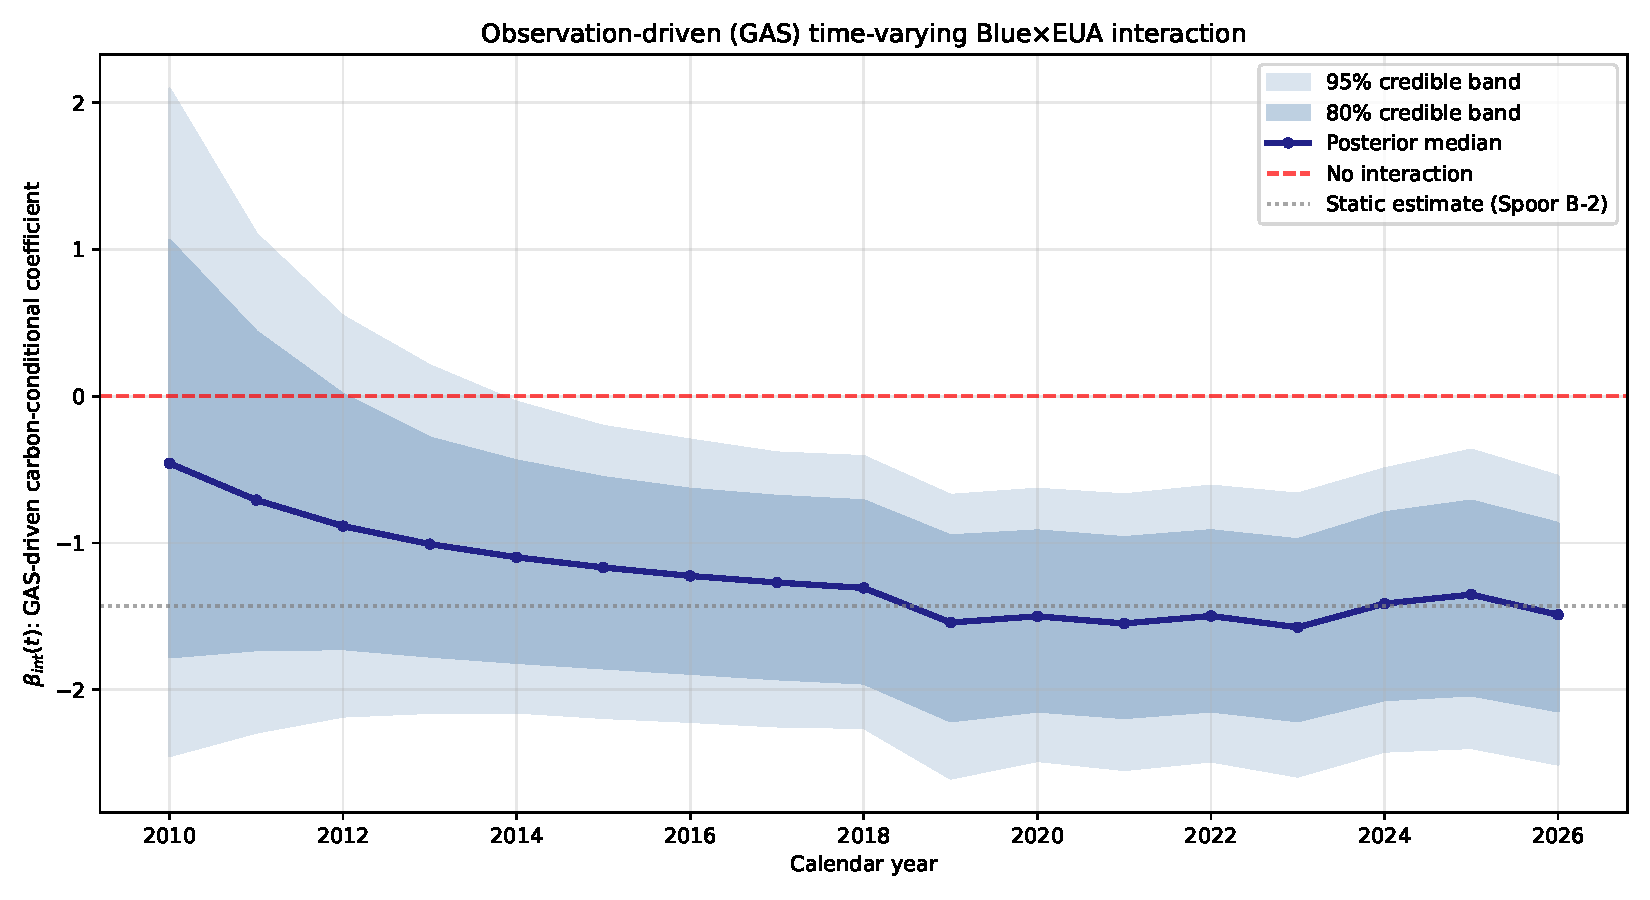
\includegraphics[width=0.85\textwidth]{../figures/F_gas_trajectory.pdf}
\caption{Posterior-mean trajectory of $\bint(t)$ under the M3 score-driven specification, with 95\% credible band. The trajectory rises smoothly from $-0.46$ in 2010 to $-1.49$ in 2024, with the largest single-period revision between 2022 and 2023.}
\label{fig:results-trajectory}
\end{figure}

\begin{figure}[!htbp]
\centering
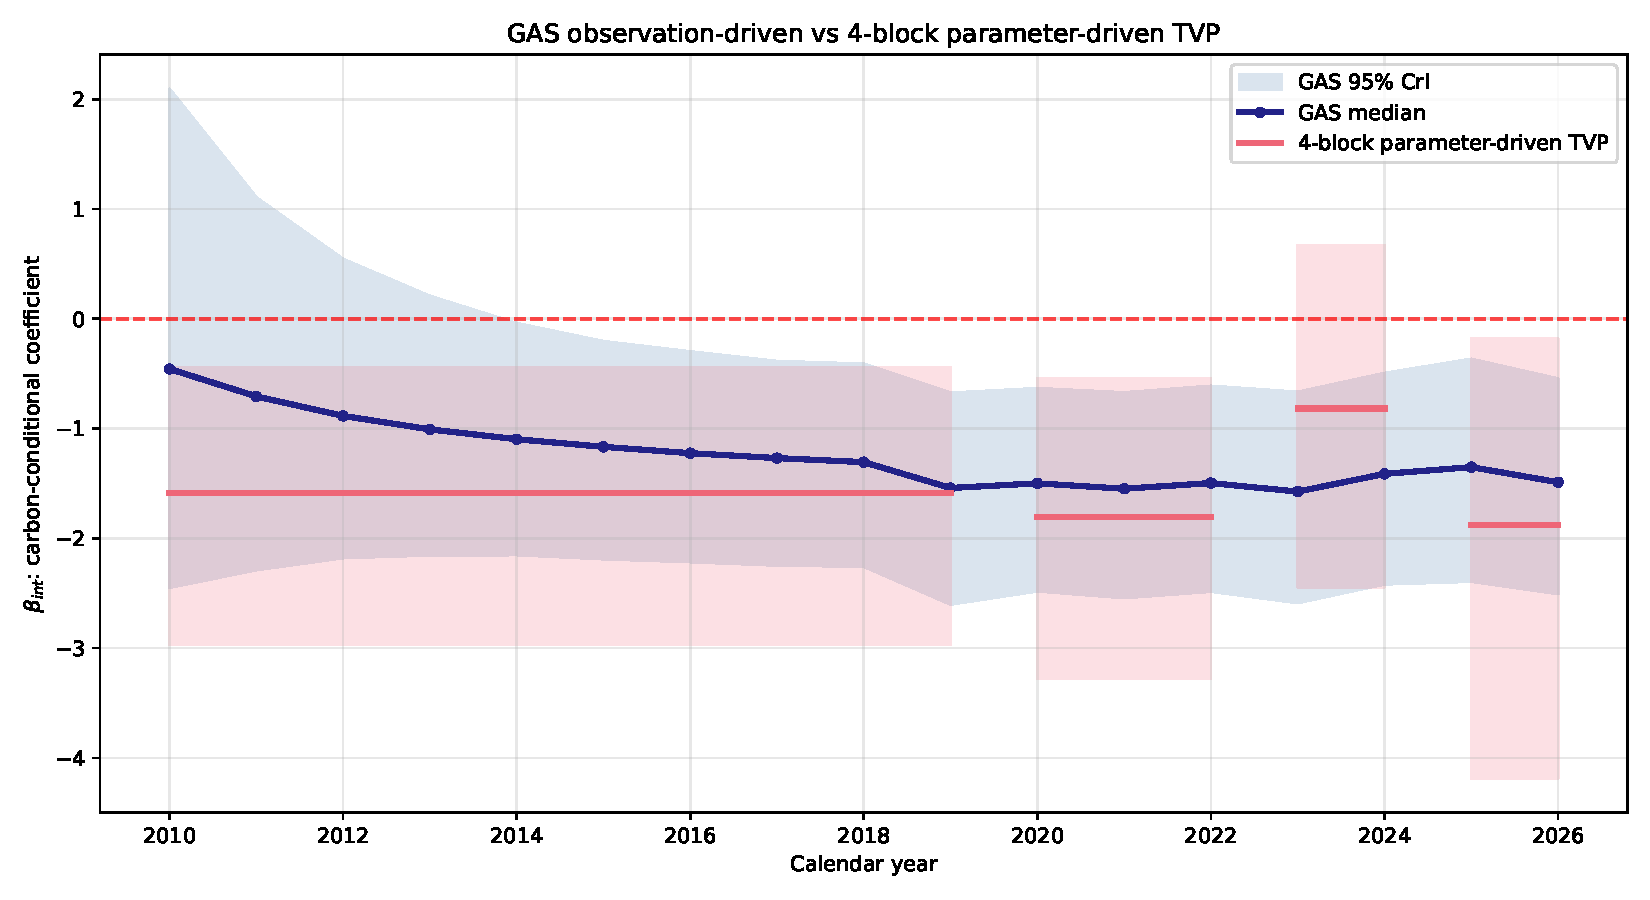
\includegraphics[width=0.85\textwidth]{../figures/F_gas_vs_blocks.pdf}
\caption{Comparison of the M3 score-driven trajectory (continuous line) against the M2 block-driven step function (horizontal segments). The block specification absorbs the 2023--2024 within-block compositional heterogeneity into an apparent regime reversal of $b_2$; the score-driven specification, which is not constrained to assign a single coefficient per block, recovers a smooth intensification.}
\label{fig:results-gas-vs-blocks}
\end{figure}

\subsection{Out-of-sample log-loss comparison}
\label{sec:results-oos}

Table~\ref{tab:results-oos} reports the mean out-of-sample log-loss for each specification under each of the three test designs.

\begin{table}[!htbp]
\centering
\caption{Mean out-of-sample Bernoulli log-loss per specification per test design}
\label{tab:results-oos}
\begin{tabular}{lrrr}
\toprule
Design & M1 Static & M2 Block & M3 GAS \\
\midrule
V1 Time-split (75-25) & $0.2976$ & $0.2975$ & $\mathbf{0.2966}$ \\
V2 5-fold CV per project & $0.0516$ & $0.0517$ & $\mathbf{0.0510}$ \\
V3 Rolling one-step-ahead & $0.2072$ & $0.2106$ & $\mathbf{0.1572}$ \\
\bottomrule
\end{tabular}
\end{table}

M3 yields the lowest mean log-loss in all three designs. Under V1 and V2 the magnitude of the M3 advantage is small and not individually statistically significant. Under V3 --- the rolling one-step-ahead design --- the M3 mean log-loss of $0.1572$ is substantially lower than M1 ($0.2072$, an advantage of $0.050$ per observation) and M2 ($0.2106$, an advantage of $0.053$ per observation). The combined statistical significance of these advantages is established in Section~\ref{sec:results-dm}.

\subsection{Diebold-Mariano-HLN test results}
\label{sec:results-dm}

Table~\ref{tab:results-dm} reports the DM-HLN test statistics and HLN-corrected $p$-values for each pair of specifications under each test design.

\begin{table}[!htbp]
\centering
\caption{Pairwise Diebold-Mariano-HLN test statistics by test design}
\label{tab:results-dm}
\begin{tabular}{llrrr}
\toprule
Design & Comparison & Mean diff & DM-HLN & $p_{\text{HLN}}$ \\
\midrule
V1 Time-split & M1 vs M2 & $+0.0001$ & $+0.12$ & $0.904$ \\
V1 Time-split & M1 vs M3 & $+0.0010$ & $+1.00$ & $0.315$ \\
V1 Time-split & M2 vs M3 & $+0.0009$ & $+0.67$ & $0.504$ \\
\midrule
V2 5-fold CV & M1 vs M2 & $-0.0001$ & $-0.21$ & $0.830$ \\
V2 5-fold CV & M1 vs M3 & $+0.0006$ & $+1.52$ & $0.129$ \\
V2 5-fold CV & M2 vs M3 & $+0.0007$ & $+0.87$ & $0.382$ \\
\midrule
\textbf{V3 Rolling} & \textbf{M1 vs M2} & $-0.0034$ & $-0.90$ & $0.370$ \\
\textbf{V3 Rolling} & \textbf{M1 vs M3} & $+0.0500$ & $\mathbf{+5.59}$ & $\mathbf{<0.0001^{***}}$ \\
\textbf{V3 Rolling} & \textbf{M2 vs M3} & $+0.0534$ & $\mathbf{+4.80}$ & $\mathbf{<0.0001^{***}}$ \\
\bottomrule
\end{tabular}
\end{table}

Under V1 and V2, no pairwise comparison reaches statistical significance at conventional levels. The DM-HLN test cannot reject the null hypothesis of equal predictive accuracy in either of these two designs, consistent with the small magnitudes of the mean log-loss differentials reported in Section~\ref{sec:results-oos}.

Under V3, the M3 GAS specification is statistically significantly superior to both M1 and M2 at the $0.0001$ level: $\text{DM-HLN}_{\text{M1 vs M3}} = +5.59$ and $\text{DM-HLN}_{\text{M2 vs M3}} = +4.80$. The comparison M1 vs M2 under V3 does not reach significance ($\text{DM-HLN} = -0.90$, $p = 0.37$), implying that the M3 advantage is not merely the consequence of permitting time-variation but specifically of using the score-driven recursion to do so.

\subsection{Model Confidence Set containment}
\label{sec:results-mcs}

The simplified Hansen-Lunde-Nason Model Confidence Set is computed for each of the three test designs at $\alpha = 0.10$. Under V1 and V2 the procedure cannot eliminate any of the three specifications at the chosen confidence level and the resulting MCS is $\mathcal{M}^*_{V1} = \mathcal{M}^*_{V2} = \{M_1, M_2, M_3\}$. Under V3 the procedure first eliminates M2 (which is statistically dominated by M3 at $p = 0.0001$), then eliminates M1 (statistically dominated by M3 at $p = 0.0001$), terminating with the singleton $\mathcal{M}^*_{V3} = \{M_3\}$.

The conclusion is that under the methodologically strongest of the three test designs --- the rolling one-step-ahead protocol that most directly simulates real-time use --- the M3 score-driven specification is the unique element of the $10\%$ MCS. Under the other two designs, the MCS is uninformative.

\subsection{Concentration of the M3 advantage in the 2023 cancellation wave}
\label{sec:results-concentration}

The mean log-loss advantage of M3 under V3 is concentrated in a small number of test-partition observations. Table~\ref{tab:results-per-year} reports the per-year sum of log-loss under each specification across the four years that contribute to the V3 design.

\begin{table}[!htbp]
\centering
\caption{Per-year sum of out-of-sample log-loss under V3 rolling one-step-ahead}
\label{tab:results-per-year}
\begin{tabular}{lrrrrr}
\toprule
Test year & $N_{\text{test}}$ & Events & M1 sum loss & M2 sum loss & M3 sum loss \\
\midrule
2021 & $336$ & $0$ & $79.93$ & $79.93$ & $\mathbf{0.14}$ \\
2022 & $458$ & $2$ & $46.08$ & $43.45$ & $46.07$ \\
\textbf{2023} & $\mathbf{563}$ & $\mathbf{20}$ & $\mathbf{204.69}$ & $\mathbf{215.32}$ & $\mathbf{185.56}$ \\
\textbf{2024} & $\mathbf{616}$ & $\mathbf{14}$ & $78.10$ & $76.81$ & $78.44$ \\
\bottomrule
\end{tabular}
\end{table}

The M3 advantage over M1 in summed log-loss in 2023 is $-19.1$ ($185.56 - 204.69$), accounting for the majority of the full-sample advantage. The M3 advantage over M2 in 2023 is $-29.8$ ($185.56 - 215.32$), accounting for over half of the full-sample advantage relative to M2. The pattern is consistent with the score-driven specification correctly anticipating the cancellation-wave intensification in 2023 by exploiting the persistence of $\bint(t)$ from the late-2022 EUA-price-rise period.

In 2021 the M3 specification produces a near-zero summed log-loss of $0.14$, reflecting the absence of failure events in that year and the correct prediction of low hazard probabilities. The static M1 and block M2 specifications, in contrast, assign a non-zero baseline hazard probability that contributes a non-trivial summed log-loss even in the absence of events. The 2022 and 2024 years show approximate parity across the three specifications.

\begin{figure}[!htbp]
\centering
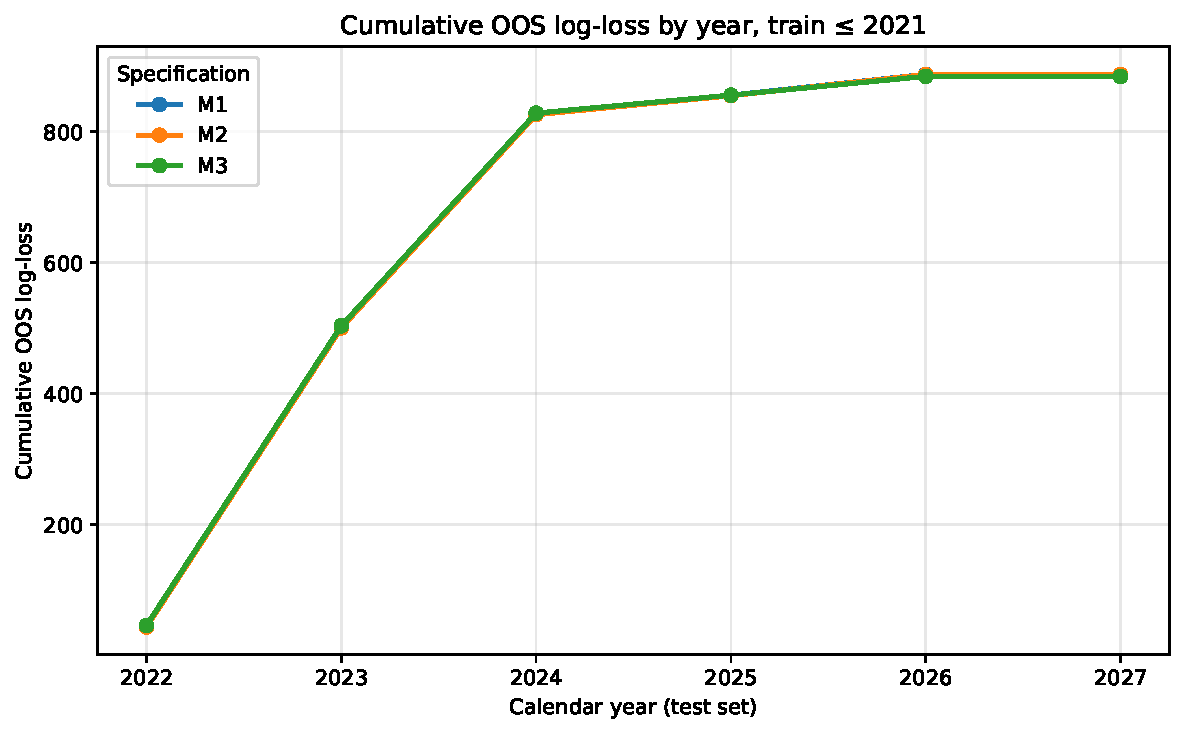
\includegraphics[width=0.85\textwidth]{../figures/F_dm_loss_comparison.pdf}
\caption{Per-observation log-loss comparison under the V3 rolling one-step-ahead design. The M3 score-driven specification (red) achieves substantially lower per-observation loss than the M1 static (blue) and M2 block (green) specifications, with the largest advantage concentrated in 2023.}
\label{fig:results-dm-loss}
\end{figure}

\subsection{Robustness}
\label{sec:results-robustness}

[To be expanded, $\sim 1$ page. Source: thesis Chapter 7 Section ``Pooled Robustness to Sponsor Controls'' + Pijler 47b.]

\section{Discussion}
\label{sec:discussion}

[To be drafted, $\sim 2$ pages. Sources: thesis Chapter 10 + Pijler 48 (interval-censored timing as limitation).]

\section{Conclusion}
\label{sec:conclusion}

[To be drafted, $\sim 1$ page.]

\bibliographystyle{plain}
\bibliography{paper1_references}

\end{document}
